\begin{surferPage}[7-gon]{منحنى من الدرجة السابعة ذو تناظر سباعي الأضلاع}
هذا المنحنى الذي يبدو مثل نجمة هو من الدرجة $7$. 
   حتى مؤخراً، كان عدد متفرداته، $84$، لا يزال أكبر عدد متفردات حقيقية معروف عنها لمنحنى من الدرجة السابعة؛ 
   ولكن في العام 2004، حطم أوليفر لابس هذا الرقم القياسي ورفعه إلى $99$.  
  
    الأوكار الثلاثة التي يمكن رؤيتها في الصورة التفاعلية ناتجة عن استعمال متعددات حدود شيبيشيف، كما في منحنى شموتوف المثمن.  
    في الواقع، هذا المنحنى على شكل نجمة هو متغاير آخر لمنحنيات شموتوف.
    هنا، تم استبدال المنحنى المسطح $T_d(x)+T_d(y)$ بسباعي أضلاع منتظم $S_7(x,y)$: 
   \[S_7(x,y) + \lambda \cdot T_d(z) = 0,\]
   مع إختيار قيمة مناسبة للامبدا  $\lambda\in\RR$. 
    \vspace*{-0.3em}
    \begin{center}
      \begin{tabular}{c@{\qquad}c}
        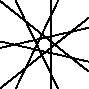
\includegraphics[height=1.5cm]{./../../common/images/labsseptic1.pdf}
        &
        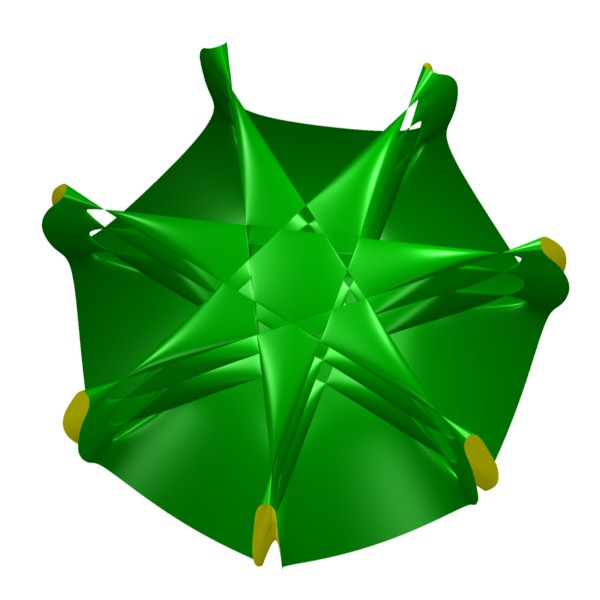
\includegraphics[height=1.5cm]{./../../common/images/septic_7eck_von_oben}
      \end{tabular}
    \end{center}
    \vspace*{-0.3em}   
    دوكو فان ستراتن (Duco van Straten) أنجز هذاالبناء المتغاير لبناء شموتوف.
\end{surferPage}
